\documentclass[12pt,a4paper]{article}

% ─── Page Layout ───────────────────────────────────────────────────────────────
\usepackage[a4paper, margin=0.8in, headheight=14pt]{geometry}

% ─── Fonts (XeLaTeX) ───────────────────────────────────────────────────────────
\usepackage{fontspec}
\usepackage{unicode-math}
\setmainfont{TeX Gyre Pagella}
\setmonofont[Scale=0.88]{TeX Gyre Cursor}
\setmathfont{Latin Modern Math}

% ─── Packages ──────────────────────────────────────────────────────────────────
\usepackage{xcolor}
\usepackage{colortbl}
\usepackage{titlesec}
\usepackage{enumitem}
\usepackage{tabularx}
\usepackage{booktabs}
\usepackage{array}
\usepackage{amsmath}
\usepackage{tikz}
\usetikzlibrary{shapes.geometric, arrows.meta, positioning, calc, fit, decorations.pathreplacing}
\usepackage{tcolorbox}
\tcbuselibrary{skins, breakable}
\usepackage{hyperref}
\usepackage{fancyhdr}
\usepackage{graphicx}
\usepackage{microtype}
\hyphenpenalty=10000
\exhyphenpenalty=10000
\sloppy
\usepackage{caption}
\usepackage{setspace}
\usepackage{multirow}
\usepackage{tocloft}

% ─── Q&A helper ────────────────────────────────────────────────────────────────
\newcommand{\Q}[1]{\textbf{#1}\par\noindent\ignorespaces}

% ─── Colour Palette ────────────────────────────────────────────────────────────
\definecolor{myred}{RGB}{196,30,58}
\definecolor{mydark}{RGB}{30,30,50}
\definecolor{mygreen}{RGB}{14,120,80}
\definecolor{myteal}{RGB}{0,130,140}
\definecolor{myamber}{RGB}{180,100,0}
\definecolor{mypurple}{RGB}{100,30,160}
\definecolor{mygray}{RGB}{246,247,249}
\definecolor{mgframe}{RGB}{180,185,200}
\definecolor{watermark}{RGB}{145,150,170}
\definecolor{hdrred}{RGB}{250,232,235}
\definecolor{hdrgreen}{RGB}{220,244,233}
\definecolor{hdrteal}{RGB}{220,242,244}
\definecolor{hdramber}{RGB}{253,242,215}
\definecolor{hdrpurple}{RGB}{238,228,255}
\definecolor{hdrgray}{RGB}{238,240,245}
\definecolor{rowalt}{RGB}{250,251,253}

% ─── Section Formatting ────────────────────────────────────────────────────────
\titleformat{\section}
  {\large\bfseries\color{myred}}{\thesection.}{0.5em}{}
  [\vspace{1pt}{\color{myred}\rule{\linewidth}{0.8pt}}]
\titleformat{\subsection}
  {\normalsize\bfseries\color{myteal}}{\thesubsection}{0.5em}{}
\titlespacing*{\section}{0pt}{18pt}{7pt}
\titlespacing*{\subsection}{0pt}{11pt}{4pt}

% ─── Paragraph ─────────────────────────────────────────────────────────────────
\setlength{\parindent}{0pt}
\setlength{\parskip}{4pt}

% ─── TOC Styling ───────────────────────────────────────────────────────────────
\renewcommand{\cfttoctitlefont}{\large\bfseries\color{myred}}
\renewcommand{\cftaftertoctitle}{\par\noindent{\color{myred}\rule{\linewidth}{0.8pt}}}
\setlength{\cftbeforetoctitleskip}{0pt}
\setlength{\cftaftertoctitleskip}{6pt}
\renewcommand{\cftsecfont}{\normalsize\bfseries\color{mydark}}
\renewcommand{\cftsecpagefont}{\normalsize\bfseries\color{mydark}}
\renewcommand{\cftsecleader}{\cftdotfill{\cftdotsep}}
\setlength{\cftbeforesecskip}{7pt}
\renewcommand{\cftsubsecfont}{\small\color{mydark}}
\renewcommand{\cftsubsecpagefont}{\small\color{mydark}}
\setlength{\cftbeforesubsecskip}{3pt}
\setlength{\cftsubsecindent}{1.4em}

% ─── Table helpers ─────────────────────────────────────────────────────────────
\renewcommand{\arraystretch}{1.45}
\setlength{\tabcolsep}{6pt}
\arrayrulecolor{mydark}
\newcolumntype{B}[1]{>{\small\bfseries\raggedright\arraybackslash}m{#1}}
\newcolumntype{Y}{>{\small\raggedright\arraybackslash}X}
\renewcommand{\tabularxcolumn}[1]{m{#1}}

% ─── Header / Footer ───────────────────────────────────────────────────────────
\pagestyle{fancy}
\fancyhf{}
\fancyhead[L]{\small\color{myred}\textbf{PE-EC702C}\;\color{mydark}--- Neural Network and Fuzzy Logic Control}
\fancyhead[R]{\small\color{myteal}\textbf{Module 2 Notes}}
\fancyfoot[C]{\small\color{mydark}\thepage}
\fancyfoot[R]{\small\color{watermark}\textit{\copyright\ Biraj}}
\renewcommand{\headrulewidth}{0.5pt}
\renewcommand{\footrulewidth}{0.3pt}

% ─── Hyperref ──────────────────────────────────────────────────────────────────
\hypersetup{
  colorlinks=true, linkcolor=myteal, urlcolor=myteal,
  pdfauthor={Biraj Sarkar},
  pdftitle={PE-EC702C --- Module 2 Notes}
}

% ─── tcolorbox styles ──────────────────────────────────────────────────────────
\tcbset{
  tikzbox/.style={
    colback=mygray, colframe=mgframe, boxrule=0.6pt, arc=4pt,
    left=8pt, right=8pt, top=6pt, bottom=6pt,
    colbacktitle=mgframe, coltitle=mydark,
    fonttitle=\small\bfseries
  },
  defbox/.style={
    colback=hdrgreen, colframe=mygreen, boxrule=0.8pt, arc=4pt,
    left=9pt, right=9pt, top=6pt, bottom=6pt,
    colbacktitle=mygreen, coltitle=white,
    fonttitle=\small\bfseries
  },
  formulabox/.style={
    colback=hdrteal, colframe=myteal, boxrule=0.8pt, arc=4pt,
    left=9pt, right=9pt, top=7pt, bottom=7pt,
    colbacktitle=myteal, coltitle=white,
    fonttitle=\small\bfseries
  },
  examplebox/.style={
    colback=hdramber, colframe=myamber, boxrule=0.8pt, arc=4pt,
    left=9pt, right=9pt, top=6pt, bottom=6pt,
    colbacktitle=myamber, coltitle=white,
    fonttitle=\small\bfseries,
    breakable
  },
  masonbox/.style={
    colback=hdrpurple, colframe=mypurple, boxrule=0.8pt, arc=4pt,
    left=9pt, right=9pt, top=6pt, bottom=6pt,
    colbacktitle=mypurple, coltitle=white,
    fonttitle=\small\bfseries
  },
  exambox/.style={
    colback=hdrpurple, colframe=mypurple, boxrule=1pt, arc=5pt,
    left=10pt, right=10pt, top=8pt, bottom=8pt,
    colbacktitle=mypurple, coltitle=white,
    fonttitle=\bfseries,
    breakable, title after break={\textbf{Frequently Asked / Viva Questions (contd.)}}}
}
\tcbset{breakable}

% ─── TikZ styles ───────────────────────────────────────────────────────────────
\tikzset{
  block/.style={rectangle, draw=myteal, fill=hdrteal,
    text width=2.2cm, align=center, minimum height=0.85cm,
    font=\small, rounded corners=3pt, line width=0.7pt},
  arrow/.style={-Stealth, thick, color=mydark},
  line/.style={thick, color=mydark}
}

% ═══════════════════════════════════════════════════════════════════════════════
\begin{document}
% ═══════════════════════════════════════════════════════════════════════════════

\begin{center}
  {\LARGE\bfseries\color{myred} PE-EC702C --- Neural Network \& Fuzzy Logic Control}\\[5pt]
  {\normalsize\color{mydark} Semester VII \quad$\bullet$\quad 3L:0T:0P \quad$\bullet$\quad 3 Credits}\\[3pt]
  {\normalsize\color{myteal}\textbf{Module 2 Exam Notes: Competitive Neural Networks}}\\[3pt]
  {\small\color{mydark} CGEC \;$|$\; B.Tech ECE (2023--27) \;$|$\; \textit{Biraj Sarkar}}
\end{center}
\vspace{2pt}
\noindent{\color{myred}\rule{\linewidth}{1.5pt}}
\vspace{2pt}

\hypersetup{linkcolor=mydark}
\tableofcontents
\hypersetup{linkcolor=myteal}
\newpage

% ===============================================================================
\section{Introduction to Competitive Learning}
% ===============================================================================

Unlike feedforward networks that update weights based on output error signals, competitive learning networks are based on a winner-take-all strategy where nodes compete with each other to become active.

\begin{tcolorbox}[defbox, title={Competitive Learning}]
\textbf{Competitive Learning} is an unsupervised learning process where output neurons compete for activation. Only one neuron (the winning neuron) remains active at a time, and its weights are updated to become more similar to the input vector.
\end{tcolorbox}

% ===============================================================================
\section{Kohonen Self-Organizing Maps (SOM)}
% ===============================================================================

Introduced by Teuvo Kohonen in 1982, the Self-Organizing Map (SOM) is an unsupervised learning network that maps high-dimensional input patterns to a low-dimensional (typically 1D or 2D) topological grid of neurons.

\begin{tcolorbox}[tikzbox, title={Kohonen Self-Organizing Map Architecture}]
\centering
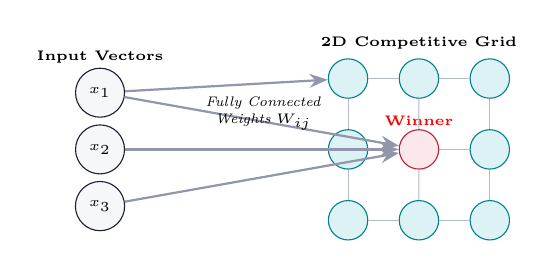
\begin{tikzpicture}[scale=0.9, every node/.style={font=\tiny}]
  % Inputs
  \node[circle, draw=mydark, fill=mygray, minimum size=0.5cm] (x1) at (-2.5, 0.8) {$x_1$};
  \node[circle, draw=mydark, fill=mygray, minimum size=0.5cm] (x2) at (-2.5, 0) {$x_2$};
  \node[circle, draw=mydark, fill=mygray, minimum size=0.5cm] (x3) at (-2.5, -0.8) {$x_3$};
  \node at (-2.5, 1.3) {\textbf{Input Vectors}};

  % 2D Grid
  \node[circle, draw=myteal, fill=hdrteal, minimum size=0.5cm] (g11) at (1, 1) {};
  \node[circle, draw=myteal, fill=hdrteal, minimum size=0.5cm] (g12) at (2, 1) {};
  \node[circle, draw=myteal, fill=hdrteal, minimum size=0.5cm] (g13) at (3, 1) {};
  \node[circle, draw=myteal, fill=hdrteal, minimum size=0.5cm] (g21) at (1, 0) {};
  \node[circle, draw=myteal, fill=hdrred, draw=myred, minimum size=0.5cm] (g22) at (2, 0) {};
  \node[circle, draw=myteal, fill=hdrteal, minimum size=0.5cm] (g23) at (3, 0) {};
  \node[circle, draw=myteal, fill=hdrteal, minimum size=0.5cm] (g31) at (1, -1) {};
  \node[circle, draw=myteal, fill=hdrteal, minimum size=0.5cm] (g32) at (2, -1) {};
  \node[circle, draw=myteal, fill=hdrteal, minimum size=0.5cm] (g33) at (3, -1) {};
  \node at (2, 1.5) {\textbf{2D Competitive Grid}};

  % Winner Highlight
  \node[red, font=\tiny\bfseries] at (2, 0.4) {Winner};

  % Grid Lines representing neighborhood
  \draw[thin, color=mgframe] (g11) -- (g12) -- (g13);
  \draw[thin, color=mgframe] (g21) -- (g22) -- (g23);
  \draw[thin, color=mgframe] (g31) -- (g32) -- (g33);
  \draw[thin, color=mgframe] (g11) -- (g21) -- (g31);
  \draw[thin, color=mgframe] (g12) -- (g22) -- (g32);
  \draw[thin, color=mgframe] (g13) -- (g23) -- (g33);

  % Connections
  \draw[arrow, color=watermark] (x1) -- (g11);
  \draw[arrow, color=watermark] (x1) -- (g22);
  \draw[arrow, color=watermark] (x2) -- (g22);
  \draw[arrow, color=watermark] (x3) -- (g22);
  
  \node at (-0.2, 0.5) [align=center, font=\tiny\itshape] {Fully Connected\\Weights $W_{ij}$};
\end{tikzpicture}
\end{tcolorbox}

\subsection{Kohonen SOM Learning Algorithm}
The training process involves four major steps:
\begin{enumerate}[leftmargin=*, itemsep=3.5pt]
  \item \textbf{Initialization:} Initialize weight vectors $W_j = (w_{j1}, w_{j2}, \ldots, w_{jn})^T$ for each grid node $j$ with small random values. Set parameters: initial learning rate $\alpha_0$ and initial neighborhood radius $\sigma_0$.
  \item \textbf{Similarity Matching (Finding the BMU):} For a given input vector $X = (x_1, x_2, \ldots, x_n)^T$, compute the Euclidean distance to all weight vectors:
    \begin{equation}
      d_j(X) = ||X - W_j|| = \sqrt{\sum_{i=1}^n (x_i - w_{ji})^2}
    \end{equation}
    Identify the winning neuron (Best Matching Unit, BMU) index $c$:
    \begin{equation}
      c = \arg\min_{j} d_j(X)
    \end{equation}
  \item \textbf{Weight Updating:} Update weights of the BMU and all neurons within its neighborhood $h_{cj}(t)$:
    \begin{equation}
      W_j(t+1) = W_j(t) + \alpha(t) h_{cj}(t) [X - W_j(t)]
    \end{equation}
  \item \textbf{Decay Parameters:} Decay the learning rate and the neighborhood size:
    \begin{equation}
      \alpha(t) = \alpha_0 \exp\left(-\frac{t}{\tau_1}\right), \quad \sigma(t) = \sigma_0 \exp\left(-\frac{t}{\tau_2}\right)
    \end{equation}
\end{enumerate}

% ===============================================================================
\section{Learning Vector Quantization (LVQ)}
% ===============================================================================

Learning Vector Quantization (LVQ), introduced by Kohonen, is a supervised competitive learning algorithm used for pattern classification.

\begin{tcolorbox}[defbox, title={LVQ Architecture}]
An \textbf{LVQ network} consists of an input layer and a competitive layer containing codebook vectors (prototype vectors). Each codebook vector is assigned a specific target class.
\end{tcolorbox}

\subsection{LVQ Update Rules}
Let $w_c$ be the codebook vector closest to the input vector $x$ (in terms of Euclidean distance). The weights are adjusted as follows:
\par\noindent
\begin{tcolorbox}[formulabox, title={LVQ Supervised Training updates}]
If the winning codebook vector $w_c$ belongs to the \textbf{correct class} as the input $x$:
\begin{equation}
  w_c(t+1) = w_c(t) + \alpha(t) [x - w_c(t)]
\end{equation}
If the winning codebook vector $w_c$ belongs to an \textbf{incorrect class} relative to input $x$:
\begin{equation}
  w_c(t+1) = w_c(t) - \alpha(t) [x - w_c(t)]
\end{equation}
All other codebook vectors remain unchanged:
\begin{equation}
  w_j(t+1) = w_j(t) \quad \text{for } j \neq c
\end{equation}
\end{tcolorbox}

% ===============================================================================
\section{Counter Propagation Networks (CPN)}
% ===============================================================================

Developed by Robert Hecht-Nielsen in 1987, CPN combines a competitive unsupervised layer (Kohonen SOM) with a self-organizing outstar layer (Grossberg outstar). It acts as a fast lookup table to approximate continuous mathematical functions.

\subsection{CPN Architecture}
CPN contains three layers: Input layer, Kohonen layer (competitive), and Grossberg (Outstar) output layer.

\begin{tcolorbox}[tikzbox, title={Counter Propagation Network (CPN) Layout}]
\centering
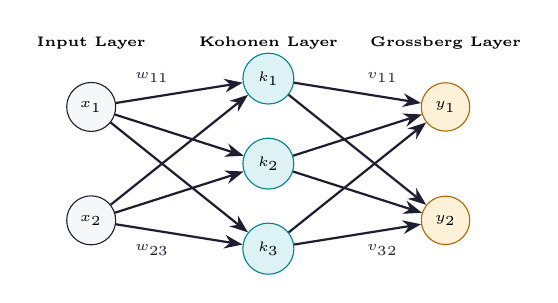
\begin{tikzpicture}[scale=0.9, every node/.style={font=\tiny}]
  % Inputs
  \node[circle, draw=mydark, fill=mygray, minimum size=0.5cm] (x1) at (-2.5, 0.8) {$x_1$};
  \node[circle, draw=mydark, fill=mygray, minimum size=0.5cm] (x2) at (-2.5, -0.8) {$x_2$};
  
  % Kohonen Nodes
  \node[circle, draw=myteal, fill=hdrteal, minimum size=0.5cm] (k1) at (0, 1.2) {$k_1$};
  \node[circle, draw=myteal, fill=hdrteal, minimum size=0.5cm] (k2) at (0, 0) {$k_2$};
  \node[circle, draw=myteal, fill=hdrteal, minimum size=0.5cm] (k3) at (0, -1.2) {$k_3$};
  
  % Grossberg Nodes
  \node[circle, draw=myamber, fill=hdramber, minimum size=0.5cm] (g1) at (2.5, 0.8) {$y_1$};
  \node[circle, draw=myamber, fill=hdramber, minimum size=0.5cm] (g2) at (2.5, -0.8) {$y_2$};

  % Connections: Input to Kohonen (Weights W)
  \draw[arrow] (x1) -- node[midway, above left] {$w_{11}$} (k1);
  \draw[arrow] (x1) -- (k2);
  \draw[arrow] (x1) -- (k3);
  \draw[arrow] (x2) -- (k1);
  \draw[arrow] (x2) -- (k2);
  \draw[arrow] (x2) -- node[midway, below left] {$w_{23}$} (k3);

  % Connections: Kohonen to Grossberg (Weights V)
  \draw[arrow] (k1) -- node[midway, above right] {$v_{11}$} (g1);
  \draw[arrow] (k1) -- (g2);
  \draw[arrow] (k2) -- (g1);
  \draw[arrow] (k2) -- (g2);
  \draw[arrow] (k3) -- (g1);
  \draw[arrow] (k3) -- node[midway, below right] {$v_{32}$} (g2);

  % Layer Labels
  \node at (-2.5, 1.7) {\textbf{Input Layer}};
  \node at (0, 1.7) {\textbf{Kohonen Layer}};
  \node at (2.5, 1.7) {\textbf{Grossberg Layer}};
\end{tikzpicture}
\end{tcolorbox}

\subsection{CPN Training phases}
\begin{enumerate}[leftmargin=*, itemsep=3pt]
  \item \textbf{First Phase (Kohonen Training):} The input vector $X$ is presented. The Kohonen layer acts as a competitive classifier. The winning neuron $c$ is determined, and its weights $W_c$ are updated using standard Kohonen rules.
  \item \textbf{Second Phase (Grossberg Training):} The Kohonen layer outputs a binary vector where only the winning unit has activation $1$, and all others are $0$ ($z_j = \delta_{jc}$). The Grossberg weights $V$ are updated to match the target vector $Y$:
    \begin{equation}
      v_{jk}(t+1) = v_{jk}(t) + \beta [y_k - v_{jk}(t)] z_j
    \end{equation}
    For the winner $c$: $V_c(t+1) = V_c(t) + \beta [Y - V_c(t)]$.
\end{enumerate}

% ===============================================================================
\section{Worked Examples}
% ===============================================================================

\begin{tcolorbox}[examplebox, title={Kohonen SOM Winning Neuron and Weight Update}]
\textbf{Problem:} Given an input vector $X = \begin{bmatrix} 0.8 & 0.6 \end{bmatrix}^T$ and three Kohonen neurons with weight vectors:
\begin{equation*}
  W_1 = \begin{bmatrix} 0.9 & 0.1 \end{bmatrix}^T, \quad W_2 = \begin{bmatrix} 0.7 & 0.5 \end{bmatrix}^T, \quad W_3 = \begin{bmatrix} 0.2 & 0.8 \end{bmatrix}^T
\end{equation*}
\begin{enumerate}[label=(\alph*), leftmargin=*, itemsep=2.5pt]
  \item Identify the winning neuron (BMU) using Euclidean distance.
  \item Update the weight vector of the winning neuron using learning rate $\alpha = 0.5$.
\end{enumerate}
\par\vspace{4pt}\noindent\rule{\linewidth}{0.5pt}\par
\textbf{Solution:}

\textbf{(a) Similarity Matching:}
Compute the squared Euclidean distance $D_j = ||X - W_j||^2$ for each neuron:
\begin{itemize}[leftmargin=*, itemsep=2pt]
  \item For $W_1$:
    \begin{equation*}
      D_1 = (0.8 - 0.9)^2 + (0.6 - 0.1)^2 = (-0.1)^2 + (0.5)^2 = 0.01 + 0.25 = 0.26
    \end{equation*}
  \item For $W_2$:
    \begin{equation*}
      D_2 = (0.8 - 0.7)^2 + (0.6 - 0.5)^2 = (0.1)^2 + (0.1)^2 = 0.01 + 0.01 = 0.02
    \end{equation*}
  \item For $W_3$:
    \begin{equation*}
      D_3 = (0.8 - 0.2)^2 + (0.6 - 0.8)^2 = (0.6)^2 + (-0.2)^2 = 0.36 + 0.04 = 0.40
    \end{equation*}
\end{itemize}
Since $D_2 = 0.02$ is the minimum, \textbf{Neuron 2 ($W_2$)} is the winning neuron (BMU).

\par\vspace{4pt}
\textbf{(b) Weight Update:}
Update the weights of the winning neuron $W_2$:
\begin{align*}
  W_2(new) &= W_2(old) + \alpha [X - W_2(old)] \\
  &= \begin{bmatrix} 0.7 \\ 0.5 \end{bmatrix} + 0.5 \left( \begin{bmatrix} 0.8 \\ 0.6 \end{bmatrix} - \begin{bmatrix} 0.7 \\ 0.5 \end{bmatrix} \right) \\
  &= \begin{bmatrix} 0.7 \\ 0.5 \end{bmatrix} + 0.5 \begin{bmatrix} 0.1 \\ 0.1 \end{bmatrix} = \begin{bmatrix} 0.7 \\ 0.5 \end{bmatrix} + \begin{bmatrix} 0.05 \\ 0.05 \end{bmatrix} = \begin{bmatrix} 0.75 \\ 0.55 \end{bmatrix}
\end{align*}
The updated weight vector is $W_2 = \begin{bmatrix} 0.75 & 0.55 \end{bmatrix}^T$.
\end{tcolorbox}

\begin{tcolorbox}[examplebox, title={LVQ Classifier Updates}]
\textbf{Problem:} Given an input vector $x = \begin{bmatrix} 0.1 & 0.9 \end{bmatrix}$ belonging to Class 1, and the closest codebook vector $w_c = \begin{bmatrix} 0.2 & 0.7 \end{bmatrix}$. 
Calculate the updated codebook vector for:
\begin{enumerate}[label=(\alph*), leftmargin=*]
  \item Class of $w_c$ is Class 1 (correct class)
  \item Class of $w_c$ is Class 2 (incorrect class)
\end{enumerate}
Assume learning rate $\alpha = 0.2$.
\par\vspace{4pt}\noindent\rule{\linewidth}{0.5pt}\par
\textbf{Solution:}

\textbf{(a) Correct Class Update (Push towards input):}
\begin{align*}
  w_c(new) &= w_c(old) + \alpha [x - w_c(old)] \\
  &= \begin{bmatrix} 0.2 \\ 0.7 \end{bmatrix} + 0.2 \left( \begin{bmatrix} 0.1 \\ 0.9 \end{bmatrix} - \begin{bmatrix} 0.2 \\ 0.7 \end{bmatrix} \right) \\
  &= \begin{bmatrix} 0.2 \\ 0.7 \end{bmatrix} + 0.2 \begin{bmatrix} -0.1 \\ 0.2 \end{bmatrix} = \begin{bmatrix} 0.2 - 0.02 \\ 0.7 + 0.04 \end{bmatrix} = \begin{bmatrix} 0.18 \\ 0.74 \end{bmatrix}
\end{align*}

\textbf{(b) Incorrect Class Update (Pull away from input):}
\begin{align*}
  w_c(new) &= w_c(old) - \alpha [x - w_c(old)] \\
  &= \begin{bmatrix} 0.2 \\ 0.7 \end{bmatrix} - 0.2 \left( \begin{bmatrix} 0.1 \\ 0.9 \end{bmatrix} - \begin{bmatrix} 0.2 \\ 0.7 \end{bmatrix} \right) \\
  &= \begin{bmatrix} 0.2 \\ 0.7 \end{bmatrix} - 0.2 \begin{bmatrix} -0.1 \\ 0.2 \end{bmatrix} = \begin{bmatrix} 0.2 + 0.02 \\ 0.7 - 0.04 \end{bmatrix} = \begin{bmatrix} 0.22 \\ 0.66 \end{bmatrix}
\end{align*}
\end{tcolorbox}

\newpage

% ===============================================================================
% MANDATORY QUICK REVISION PAGE
% ===============================================================================
\begin{center}
  {\large\bfseries\color{myred} Quick Revision --- Module II}\\[3pt]
  {\small\color{mydark} Competitive Neural Networks $|$ PE-EC702C}
\end{center}
\noindent{\color{myred}\rule{\linewidth}{1.2pt}}
\vspace{4pt}

\begin{tcolorbox}[formulabox, title={\textbf{Key Formulas at a Glance}}]
\renewcommand{\arraystretch}{1.3}
\begin{tabularx}{\linewidth}{B{5.0cm} X}Euclidean Distance in SOM & $d_j(X) = \sqrt{\sum_{i=1}^n (x_i - w_{ji})^2}$ \\
Winning Neuron (BMU) Index & $c = \arg\min_j d_j(X)$ \\
Kohonen Weight Update & $W_j(t+1) = W_j(t) + \alpha(t) h_{cj}(t) [X - W_j(t)]$ \\
LVQ Correct Update & $w_c(t+1) = w_c(t) + \alpha(t) [x - w_c(t)]$ \\
LVQ Incorrect Update & $w_c(t+1) = w_c(t) - \alpha(t) [x - w_c(t)]$ \\
Grossberg outstar Update & $V_c(t+1) = V_c(t) + \beta [Y - V_c(t)]$
\end{tabularx}
\end{tcolorbox}

\begin{tcolorbox}[defbox, title={\textbf{One-Line Definitions}}]
\begin{itemize}[leftmargin=*, itemsep=2.5pt, topsep=0pt]
  \item \textbf{Kohonen SOM:} An unsupervised clustering network that creates a topology-preserving mapping of high-dimensional input features.
  \item \textbf{Best Matching Unit (BMU):} The neuron in a competitive layer whose weight vector is closest to the current input vector.
  \item \textbf{LVQ:} A supervised competitive network that uses prototype vectors to map inputs to specific classification boundaries.
  \item \textbf{CPN:} A hybrid network that maps input patterns to target vectors rapidly by combining a Kohonen layer with a Grossberg layer.
  \item \textbf{Grossberg Outstar:} A learning unit designed to output a specific analog target pattern when triggered by a Kohonen node.
\end{itemize}
\end{tcolorbox}

\begin{tcolorbox}[exambox, title={\textbf{Frequently Asked / Viva Questions}}]
\begin{enumerate}[leftmargin=*, itemsep=3.5pt, label=\arabic*.]
  \item \Q{What is the primary difference between Perceptron learning and Kohonen learning?} Perceptron learning is supervised and minimizes output error feedback. Kohonen learning is unsupervised and uses similarity metrics to cluster features.
  \item \Q{How does the neighborhood function $h_{cj}(t)$ change during SOM training?} It starts wide to organize the global structure of the map, and then shrinks exponentially over time to allow fine-tuning of local weights.
  \item \Q{Why is LVQ considered a supervised learning algorithm while SOM is unsupervised?} SOM groups data based solely on input similarities without class labels. LVQ adjusts its codebook vectors based on class labels to optimize classification boundaries.
  \item \Q{Explain the role of Grossberg outstar layer in Counter Propagation Networks.} The Kohonen layer maps inputs to a single active winning unit. The Grossberg layer acts as a lookup table, outputting a stored target vector associated with that unit.
  \item \Q{What is the significance of the vigilance parameter in competitive networks?} It controls the sensitivity of node matching. In networks like ART, it determines if a new cluster must be created or if the input fits an existing cluster.
  \item \Q{Why does CPN train faster than Backpropagation networks?} CPN updates only the winning Kohonen neuron and the corresponding Grossberg weights, avoiding expensive error propagation across multiple layers.
  \item \Q{What is the purpose of lateral inhibition in competitive networks?} It allows active neurons to suppress the activation of neighboring competitive neurons, ensuring that only one winning neuron (the BMU) remains active.
  \item \Q{How does LVQ-2 differ from standard LVQ-1?} LVQ-1 updates only the single closest codebook vector. LVQ-2 updates the two closest vectors simultaneously if the input falls near the decision boundary.
  \item \Q{What is meant by a topology-preserving mapping in SOM?} It means that input vectors that are close in the high-dimensional feature space are mapped to neurons that are close to each other on the 2D output grid.
  \item \Q{What is the codebook vector in Learning Vector Quantization?} It is a prototype vector representing a class cluster center in the input space.
\end{enumerate}
\end{tcolorbox}

\begin{tcolorbox}[tikzbox, title={Comparison of Competitive Networks}]
\centering
{\renewcommand{\arraystretch}{1.55}%
\begin{tabularx}{\linewidth}{|>{\bfseries}B{3.2cm}|Y|Y|Y|}
\hline
Attribute & Kohonen SOM & LVQ & CPN \\
\hline
Learning Type & Unsupervised & Supervised & Hybrid (Supervised + Unsupervised) \\
\hline
Primary Application & Dimensionality reduction & Pattern classification & Function approximation \\
\hline
Output Layer Grid & 1D or 2D grid structure & 1D array of vectors & 1D array of output nodes \\
\hline
Weight Updates & Updates winner + neighbors & Updates winner only & Updates winner only \\
\hline
\end{tabularx}}
\end{tcolorbox}

\end{document}
